% Copyright 2018-2022 FIUS
%
% This file is part of theo-vorkurs-folien.
%
% theo-vorkurs-folien is free software: you can redistribute it and/or modify
% it under the terms of the GNU General Public License as published by
% the Free Software Foundation, either version 3 of the License, or
% (at your option) any later version.
%
% theo-vorkurs-folien is distributed in the hope that it will be useful,
% but WITHOUT ANY WARRANTY; without even the implied warranty of
% MERCHANTABILITY or FITNESS FOR A PARTICULAR PURPOSE.  See the
% GNU General Public License for more details.
%
% You should have received a copy of the GNU General Public License
% along with theo-vorkurs-folien.  If not, see <https://www.gnu.org/licenses/>.

\begin{frame}{Mengenoperationen - Schnitt}
    \begin{columns}
        \column{0.5\textwidth}
        \begin{alertblock}{Schnitt - $A\cap B$}
            Gegeben zwei Mengen A und B.\\
            In der Schnittmenge liegt alles, das in Menge A \textbf{und} in Menge B ist.
        \end{alertblock}
        \column{0.5\textwidth}
        \begin{figure}
            \centering
            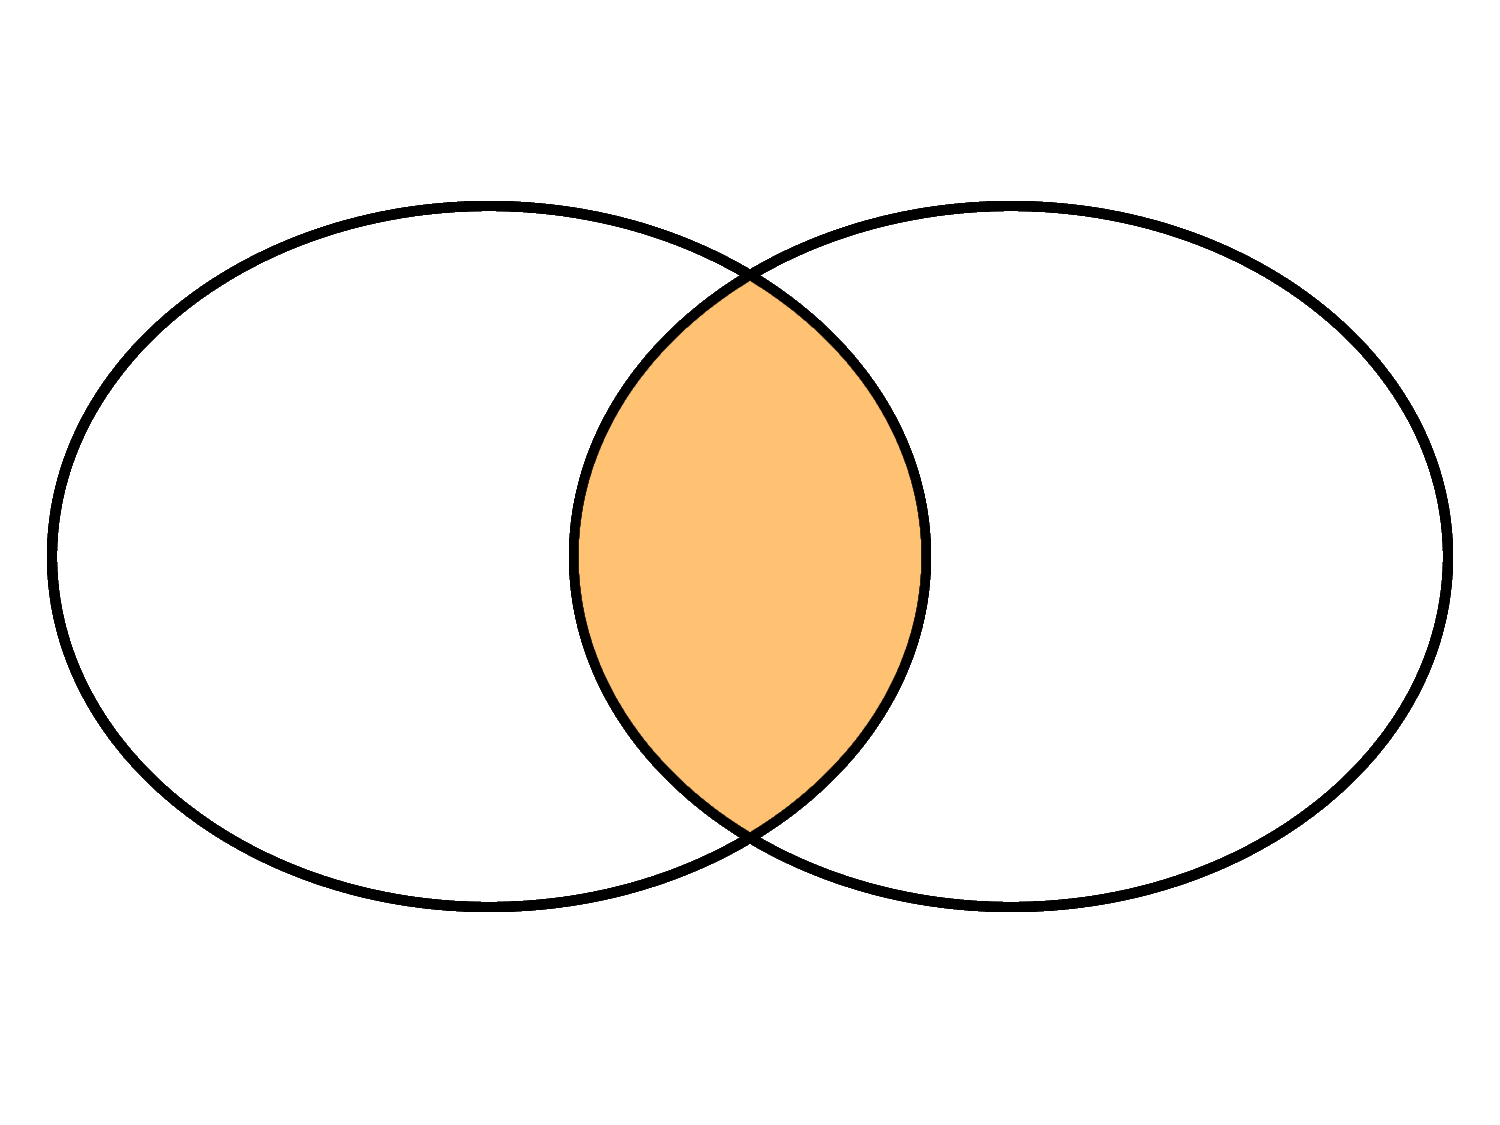
\includegraphics[width=0.7\textwidth]{../figures/AundB.png}
            \caption{Veranschaulichung der Schnittmenge}
            \label{fig:my_label}
        \end{figure}
    \end{columns}
\end{frame}

\begin{frame}{Mengenoperationen - Vereinigung}
    \begin{columns}
        \column{0.5\textwidth}
        \begin{alertblock}{Vereinigung - $A\cup B$}
            Gegeben zwei Mengen A und B.\\
            In der Vereinigung liegt alles, das nur in A, nur in B \textbf{oder} in beiden Mengen liegt.
        \end{alertblock}
        \column{0.5\textwidth}
        \begin{figure}
            \centering
            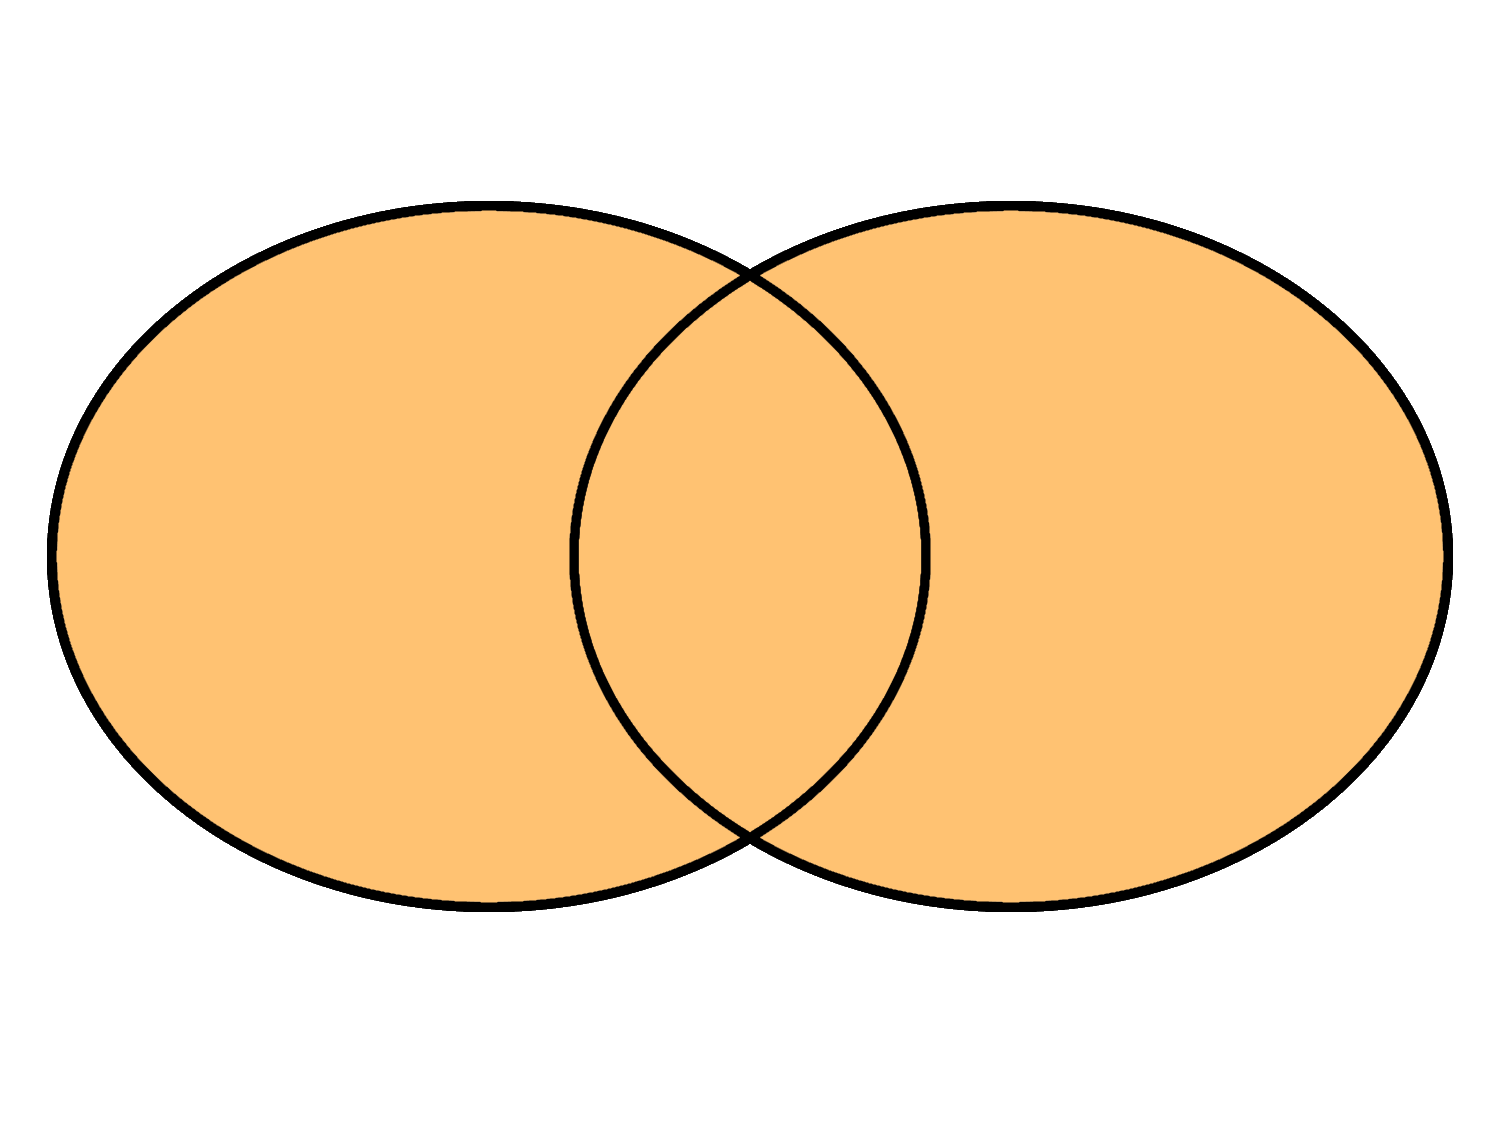
\includegraphics[width=0.7\textwidth]{../figures/AoderB.png}
            \caption{Veranschaulichung der Vereinigung}
            \label{fig:my_label}
        \end{figure}
    \end{columns}
\end{frame}

\begin{frame}{Mengenoperationen - Komplement}
    \begin{columns}
        \column{0.5\textwidth}
        \begin{alertblock}{Komplement - $\overline{A}$}
            Gegeben sei eine Menge A.\\
            Im Komplement der Menge A liegen alle Elemente, die in der Obermenge (z.B. $\mathbb{N}$), aber nicht in der Menge A selbst liegen.
        \end{alertblock}
        \column{0.5\textwidth}
        \begin{figure}
            \centering
            \begin{tikzpicture}[align=center]
    \node[
        ellipse, draw, minimum height = 2.5cm, minimum width = 4cm, fill = orange!45!white, line width = 0.25mm
    ] at (0,0) {$\overline{A}$};
    \node[
        ellipse, draw, minimum height = 1.2 cm, minimum width = 1.2cm, fill = white, line width = 0.25mm
    ] at (1cm,0) {$A$};
    \node[] at (2cm, -1cm) {$\mathbb{N}$};
\end{tikzpicture}
            \caption{Veranschaulichung des Komplements}
            \label{fig:komplement}
        \end{figure}
    \end{columns}
    \onslide<2>{\alert{\emph{Anmerkung:}} Kann auch geschrieben werden als $\mathbb{N}\setminus A$. \\
        \hspace{2cm}(gesprochen $\mathbb{N}$ \emph{\glqq ohne\grqq} $A$)}
\end{frame}

{\setbeamercolor{palette primary}{bg=ExColor}
\begin{frame}{Mengenoperationen}
    Berechne folgende Mengen
    \metroset{block=fill}
    \begin{alertblock}{Normal}
        \begin{itemize}
            \item $M_1 = \{1\}\cup \{2\}$
            \item $M_2 = \{\} \cap \{-1, 0, 1\}$
            \item $M_3 = \mathbb{N} \cup \mathbb{Z}$
            \item $M_4 = \overline{\{3^{n}\mid n \ \text{ist gerade}\} }$ über $\mathbb{N}$
        \end{itemize}
    \end{alertblock}
    \begin{alertblock}{Schwer bis sehr schwer}
        \begin{itemize}
            \item $M_5 = \{1, 2, 3\} \cap  \{1, \{2, 3\}\}$
            \item $M_6 = \{u \mid |u| \equiv 0 \pmod 2, u \in \mathbb{N}\}$\\\hspace{0.65cm}$\cup$ $\{v \mid |v| \equiv 0 \pmod 4, v \in \mathbb{N}\}$
            \item $M_7 = \overline{\{a^{n} \mid n \ \text{ist gerade}, a \in \{3,4\}\}}$ über $\mathbb{N}$
        \end{itemize}
    \end{alertblock}
\end{frame}

\begin{frame}<handout:0>{Lösungen}
    \begin{itemize}[<+- | alert@+>]
        \item
              $M_1 = \{1, 2\}$
        \item
              $M_2 = \emptyset$
        \item
              $M_3 = \mathbb{Z}$
        \item
              $M_4 = \{3^{n} \mid$ n ist ungerade$\}$
        \item
              $M_5 = \{1\}$
        \item
              $M_6 = \{u \mid |u| \equiv 0 \pmod 2, u \in \mathbb{N}\}$
        \item
              $M_7 = \mathbb{N} \setminus \{9^n, 16^n \mid n \in \mathbb N\}$\\
              \hspace{0.44cm}$ = \mathbb{N} \setminus \{3^{2n}, 4^{2n} \mid n \in \mathbb N\}$
    \end{itemize}
\end{frame}
}
